\documentclass[tikz]{standalone}
\usepackage{tikz-feynman}
\usetikzlibrary{calc}

\begin{document}
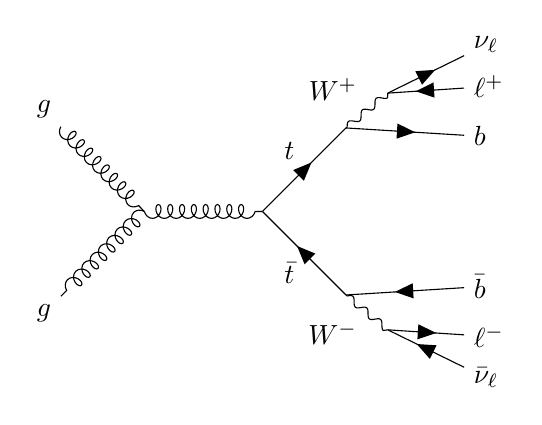
\begin{tikzpicture}
  \begin{feynman}
    % Define vertices
    \vertex (g1);
    \vertex [right = of g1] (i1_1);
    \vertex [above left = of g1] (i1) {$g$};
    \vertex [below left = of g1] (i2) {$g$};

    \vertex [above right = of i1_1] (top);
    \vertex [below right = of i1_1] (tbar);
    \vertex [right = of top, yshift = -3pt] (b) {$b$};
    \vertex [right = of tbar, yshift = 3pt] (bbar) {$\bar{b}$};

    \vertex [right = of top, yshift = 30pt] (nu_l) {$\nu_\ell$};
    \vertex [right = of top, yshift = 15pt] (anti_lep) {$\ell^+$};
    
    \vertex [right = of tbar, yshift = -30pt] (anti_nu_l) {$\bar{\nu}_\ell$};
    \vertex [right = of tbar, yshift = -15pt] (lep) {$\ell^-$};

    \vertex [above right = of top, yshift = -5pt] (W_helper_1);
    \vertex [below right = of tbar, yshift = 5pt] (W_helper_2);

    \vertex at ($(top)!0.5!(W_helper_1)$) (W_plus);
    \vertex at ($(tbar)!0.5!(W_helper_2)$) (W_minus);




    % Draw edges
    \diagram* {
        (i1) -- [gluon] (g1) -- [gluon] (i2);
        (g1) -- [gluon] (i1_1);
        (bbar) -- [fermion ] (tbar) -- [fermion, edge label = $\bar{t}$] (i1_1) -- [fermion, edge label = $t$] (top) -- [fermion] (b);
        (top) -- [boson, edge label = $W^+$] (W_plus);
        (anti_lep) -- [fermion] (W_plus) -- [fermion] (nu_l);
        (tbar) -- [boson, edge label' = $W^-$] (W_minus);
        (anti_nu_l) -- [fermion] (W_minus) -- [fermion] (lep);
    };
  \end{feynman}
\end{tikzpicture}
\end{document}